\documentclass[../TDE6_rsf.tex]{subfiles}%

\begin{document}
\section[s]"2"{Exploitation d'un oscillogramme en RSF}
\enonce{%
	On considère le circuit ci-dessous. On pose $e(t) = E_m\cos(\wt)$ et $u(t) =
		U_m\cos(\wt+\f)$. La figure ci-dessous représente un oscillogramme réalisé à la
	fréquence $f = \SI{1.2e3}{Hz}$, avec $R = \SI{1.0}{k\Omega}$ et $C =
		\SI{0.10}{\micro F}$.
	\smallbreak
	\noindent
	\begin{isd}
		\begin{center}
			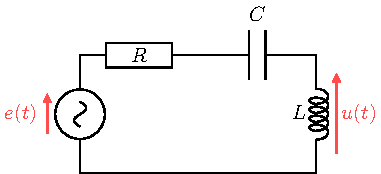
\includegraphics[width=\linewidth]{rcl_rsf}
		\end{center}
		\tcblower
		\begin{center}
			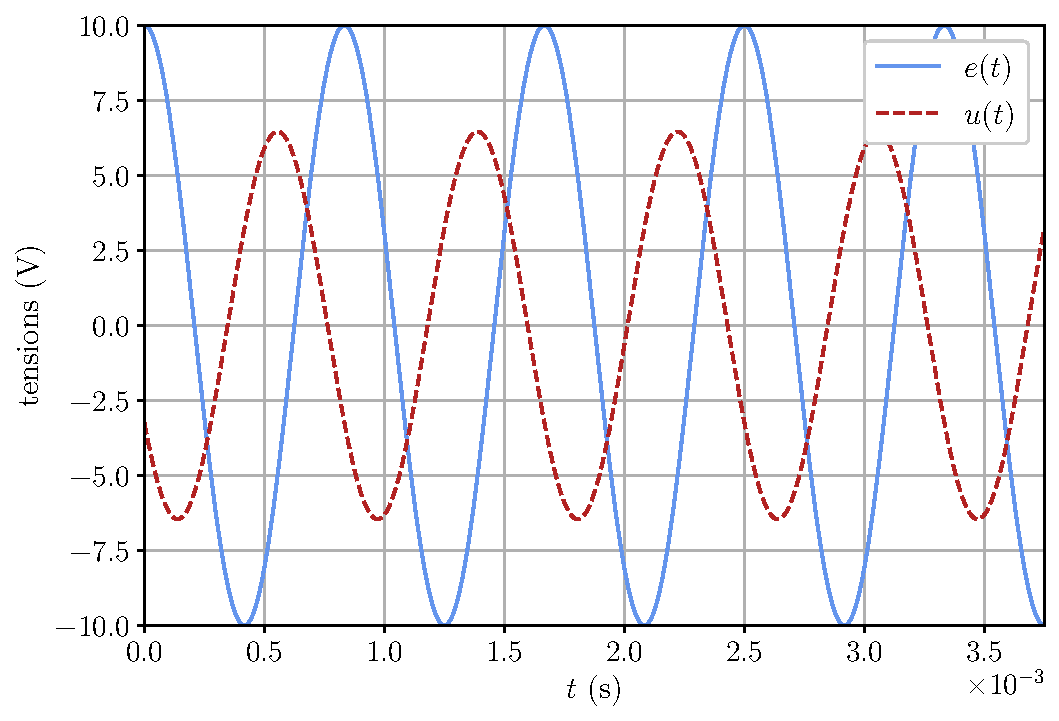
\includegraphics[width=\linewidth]{rcl_Ul_time}
		\end{center}
	\end{isd}
}
\vspace{-15pt}

\QR{%
	Déduire de cet oscillogramme les valeurs expérimentales de $E_m$,
	$U_m$ et $\f$.
}{%
	On lit l'amplitude de $e(t)$ à son maximum pour avoir \fbox{$E_m =
			\SI{10}{V}$}. On lit l'amplitude de $u(t)$ à son maximum pour avoir
	\fbox{$U_m = \SI{6}{V}$}. Pour la phase \textbf{à l'origine des temps},
	on regarde le signal à $t = 0$~: on lit $u(0) = U_m\cos(\f) =
		\SI{-3}{V}$, soit
	\begin{gather*}
		\boxed{\cos(\f) = \frac{u(0)}{U_m}}
		\qavec
		\left\{
		\begin{array}{rcl}
			u(0) & = & \SI{-3}{V} \\
			U_m  & = & \SI{6}{V}
		\end{array}
		\right.\\
		\mathrm{A.N.~:}\quad
		\boxed{\f = \frac{2\pi}{3}\si{rad}}
	\end{gather*}
}

\QR{%
Exprimer $U_m$ et $\f$ en fonction des composants du circuit et de la
pulsation $\w$. Donner l'intervalle d'existence de $\f$ et ses limites. Tracer
alors l'allure des deux graphiques $U_m(\w)$ et $\f(\w)$.
}{%
On utilise un pont diviseur de tension pour avoir l'amplitude complexe~:
\smallbreak
\noindent
\begin{isd}
	\begin{center}
		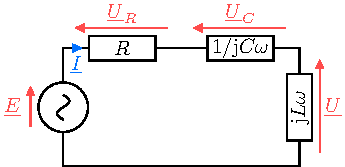
\includegraphics[width=\linewidth]{rcl_rsf-cplx}
	\end{center}
	\tcblower
	\begin{gather*}
		\Uu
		= \frac{\Zu_L}{\Zu_R + \Zu_C + \Zu_L}E_m
		\Lra
		\Uu
		= \frac{1}{\frac{\Zu_R}{\Zu_L} + \frac{\Zu_C}{\Zu_L}
			+ \frac{\Zu_L}{\Zu_L}}E_m
		\\\Lra
		\Uu
		= \frac{1}{1 + \frac{R}{\jj L\w} + \frac{1}{\jj^2\w^2CL}}E_m\\
		\Lra
		\boxed{ \Uu
			= \frac{1}{1 -\jj \frac{R}{L\w} - \frac{1}{\w^2LC}}E_m
		}
	\end{gather*}
\end{isd}
On peut en vérifier l'homogénéité en se souvenant des résultats des chapitres
précédents~:
\begin{gather*}
	\w_0{}^2 = \frac{1}{LC}
	\qdonc
	\w^2LC \text{ adimensionné}
	\qet
	\frac{R}{L} = \tau^{-1}
	\qdonc
	\frac{R}{L\w} \text{ adimensionné}
\end{gather*}
D'une manière générale, on exprimera les résultats de la sorte, avec une
fraction dont le numérateur est homogène à la quantité exprimée alors
que le dénominateur est adimensionné. \bigbreak
On trouve l'amplitude réelle en prenant le module de cette expression~:
\begin{gather*}
	U_m
	= \abs{ \Uu }
	\Lra
	\boxed{U_m
		= \frac{E}{\sqrt{\left(1 - \frac{1}{LC\w^2}\right)^2 +
				\frac{R^2}{L^2\w^2}}}
	}
\end{gather*}
On trouve la phase en en prenant l'argument~:
\begin{gather*}
	\f
	= \arg{\Uu}
	= \underbracket[1pt]{\cancel{\arg{E}}}_{=0}
	- \arg*{1 - \frac{1}{LC\w^2} - \jj \frac{R}{L\w}}
	= - \psi
\end{gather*}
Ici, il n'est pas évident de prendre l'arctangente de la tangente~: la
partie réelle de l'argument calculé n'est pas forcément positif (il
l'est si $\w^2 > \frac{1}{LC}$).
Pour faciliter l'étude de l'argument, notons $\psi = \arg*{1 -
		\frac{1}{LC\w^2} - \jj \frac{R}{L\w}}$. On alors~:
\smallbreak
\noindent
\begin{isd}
	\tcbsubtitle{\fatbox{$\w\to 0$}}
	\[
		\left\{
		\begin{array}{rcl}
			\Re(\psi) & \to & -\infty < 0
			\\
			\Im(\psi) & \to & -\infty < 0
		\end{array}
		\right.
		\Ra
		\psi \in \left[ - \pi\,; -\frac{\pi}{2} \right]
	\]
	\tcblower
	\tcbsubtitle{\fatbox{$\w\to\infty$}}
	\[
		\left\{
		\begin{array}{rcl}
			\Re(\psi) & \to & 1 > 0
			\\
			\Im(\psi) & \to & 0
		\end{array}
		\right.
		\Ra
		\psi \in \left[ - \frac{\pi}{2}\,; \frac{\pi}{2} \right]
	\]
\end{isd}
On détermine les valeurs limites en étudiant $\tan(\psi)$~:
\begin{gather*}
	\tan(\psi)
	= -\frac{R}{L\w}\times \frac{1}{1 - \frac{1}{LC\w^2}}
	= \frac{RC\w}{1 - LC\w^2}
\end{gather*}
\noindent
\begin{isd}
	\tcbsubtitle{\fatbox{$\w\to 0$}}
	\[
		\tan(\psi) \opto{}{\w\to 0} \to 0
		\Lra
		\boxed{\psi \opto{}{\w\to 0} -\pi}
	\]
	\tcblower
	\tcbsubtitle{\fatbox{$\w\to\infty$}}
	\[
		\tan(\psi) \opto{}{\w\to\infty} \to 0
		\Lra
		\boxed{\psi \opto{}{\w\to\infty} 0}
	\]
\end{isd}
Ainsi, on a les résultats opposés pour $\f = -\psi$~:
\[
	\boxed{\f \in \left] 0\,;\pi \right[}
	\qav
	\boxed{\f \opto{}{\w\to 0} \pi}
	\qet
	\boxed{\f \opto{}{\w\to\infty} 0}
\]
\noindent
\begin{isd}
	\begin{center}
		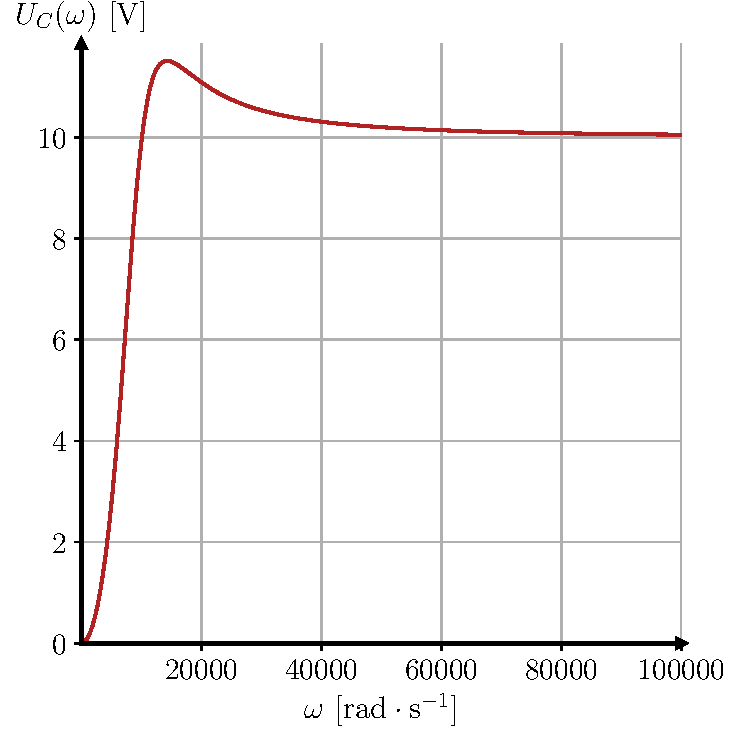
\includegraphics[width=\linewidth]{rcl_Ul_ampl_prof}
	\end{center}
	\tcblower
	\begin{center}
		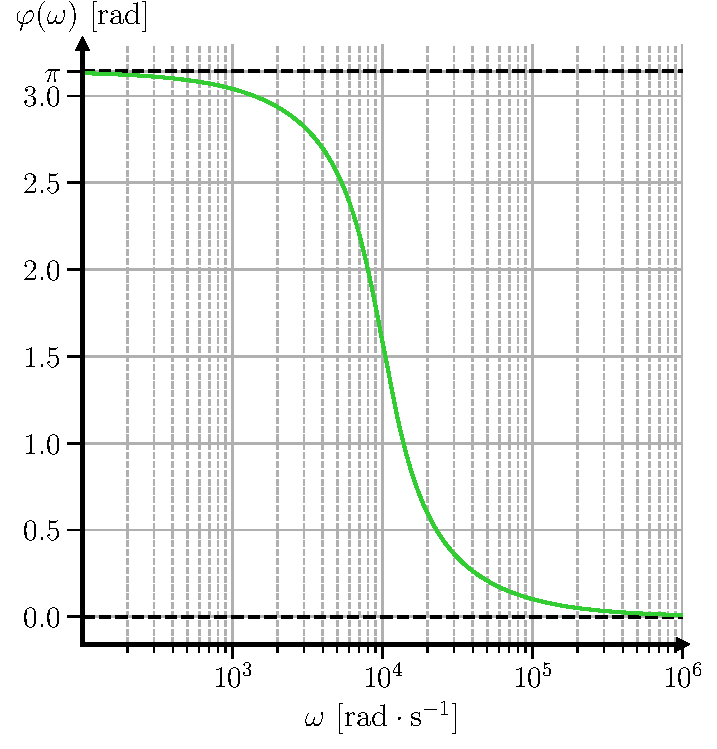
\includegraphics[width=\linewidth]{rcl_Ul_arg_prof}
	\end{center}
\end{isd}
}

\QR{%
	En déduire la valeur numérique de l'inductance $L$ de la bobine.
}{%
	Il paraît évidemment plus simple de calculer $L$ à partir de la phase,
	sachant qu'on a déterminé $\f$ à la première question~:
	\begin{gather*}
		LC\w^2 - 1
		= \frac{RC\w}{\tan(\f)}
		\Lra
		LC\w^2 = 1 + \frac{RC\w}{\tan(\f)}\\
		\Lra
		\boxed{L = \frac{1}{C\w^2} + \frac{R}{\w\tan(\f)}}
		\qavec
		\left\{
		\begin{array}{rcl}
			C  & = & \SI{0.10}{\micro F}    \\
			\w & = & 2\pi f                 \\
			f  & = & \SI{1.2e3}{Hz}         \\
			R  & = & \SI{1}{k\Omega}        \\
			\f & = & \frac{2\pi}{3}\si{rad}
		\end{array}
		\right.\\
		\mathrm{A.N.~:}\quad
		\boxed{L = \SI{9.9e-2}{H}}
	\end{gather*}
}

\end{document}
